%% The following is a directive for TeXShop to indicate the main file
%%!TEX root = diss.tex

\chapter{Case Study \#2 TKC}
\label{ch:CaseStudy2}

%In all cases these are first guesses at what needs to be in each section more or less detail need to be added.



\section{Overview of Deposits}
\label{sec:Overview of Deposits:TKC}
%
%Kimberlite Complex
%Two anomalies, focusing on the southern one (DO27)
%
%Magnetic Anomaly. Remanent magnetization is likely present but largely in the direction of the earth's field
%Density Anomaly. 
\section{Discussion of the Geophysical Data Given}
\label{sec:Discussion of the Geophysical Data Given:TKC}
%
%Magnetics: Three different surveys\\
%Gravity: Ground mag (of usable but dubious quality), Gravity Gradiometry airborne data
%
%much EM as well, outside the scope of this Master's Thesis

\section{What Information is Available}
\label{sec:What Information is Available:TKC}

%Great deal of borehole data with rock units at each depth
%We also have Phys Props at various points along the holes. We can either mean these across the facies or take the value of each facies that the specially nearest the the measured result.
%
%From the borehole data we also have created a surface model of each of the units
%
%again from the borehole data, we have graphical cross section maps

\section{Synthetic Model}
\label{sec:Synthetic Model:TKC}
%
Given the amount of \emph{a priori} information that has been collected in the region we can make a fairly non-trivial synthetic model to test various forms of constraints. The primary source of information for the creation of the synthetic model are drill hole logs of the kimberlite pipe \cite{eggleston2014peregrine}. From these drill holes, a data set representing the outer surface of the main geological units (PK and HK), was created. These are shown in \autoref{fig:TKCdataPKHK} along with the VTEM magnetic data over top of DO27, and the mesh used throughout the rest of this section. The of Earth's field in the location has an inclination of 83\degree and a declination of 19\degree.
%
\begin{figure} [h]
   \centering
   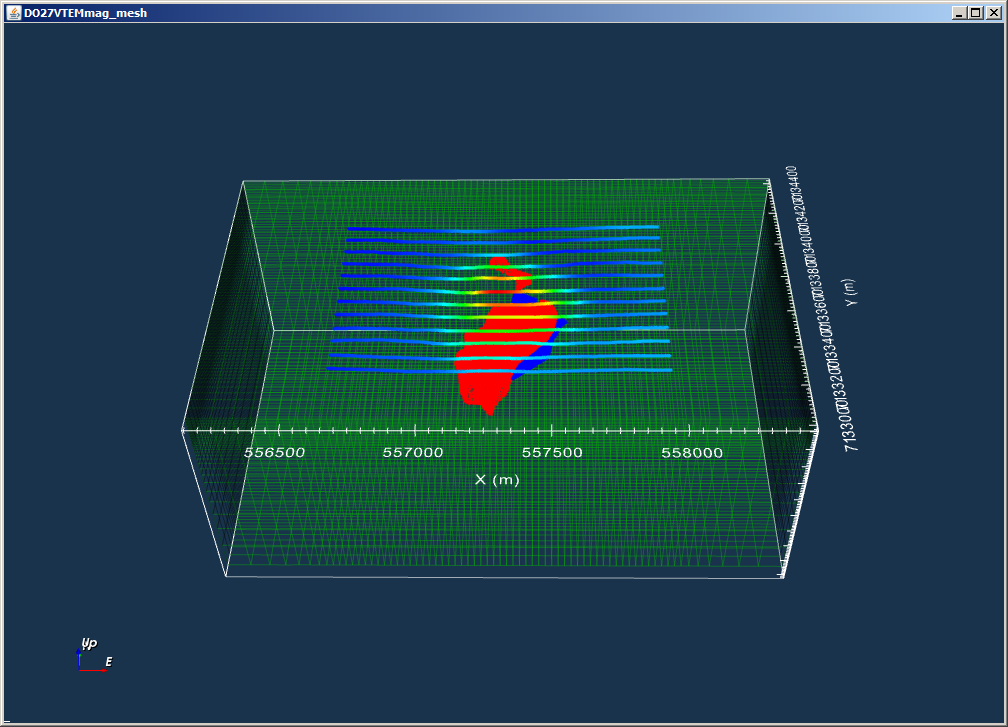
\includegraphics[width=0.8\textwidth]{images/TKC/TKCdataPKHK.PNG}
   \caption{Mesh used in this chapter along VTEM data, and outer bound of PK (blue) and HK (red)}
   \label{fig:TKCdataPKHK}
\end{figure}
%

\begin{figure} [h]
   \centering
   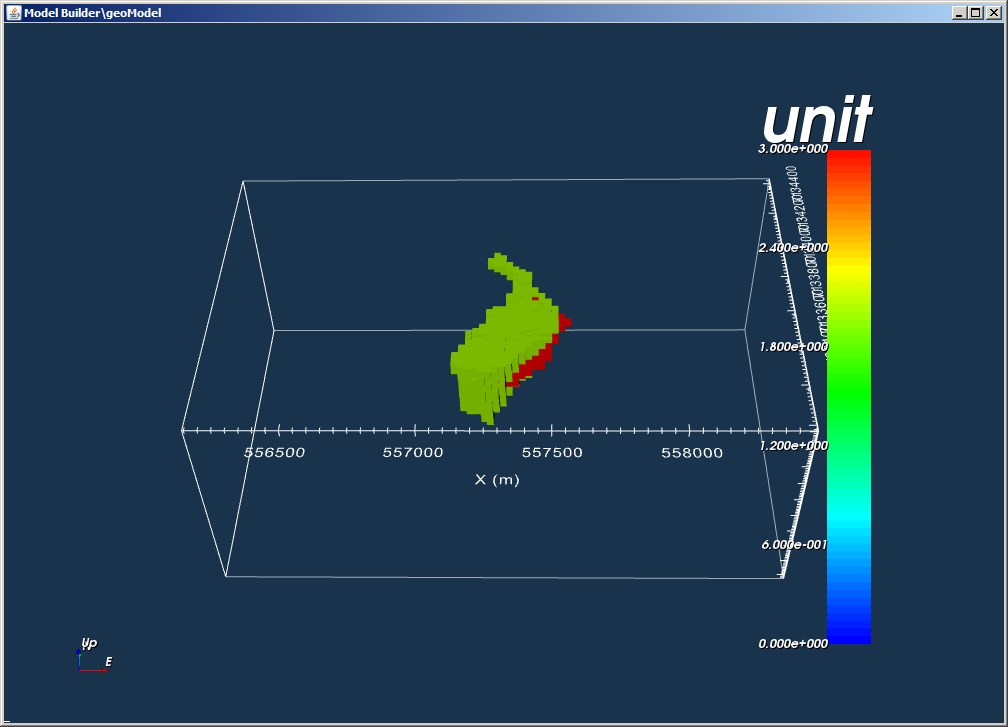
\includegraphics[width=0.8\textwidth]{images/TKC/TKCgeoModel.PNG}
   \caption{Geology model defined by geology data sets}
   \label{fig:TKCgeoModel}
\end{figure}

Using the geology unit data sets and a geological model is created \autoref{fig:TKCgeoModel}. Given this geology model and using a magnetization vector voxel-parametric inversion we now have a magnetization model that closely matches known geological structure and makes an attempt at fitting the data \autoref{fig:TKCgeoModel}. For this parametric inversion result the PK unit has an effective susceptibility of 3.28E-3 (SI) and the HK unit has an effective susceptibility of .032 (SI). These numbers may seem high but it is important to note that they are effective susceptibilities and not true susceptibilities. 

\begin{figure} [h]
   \centering
   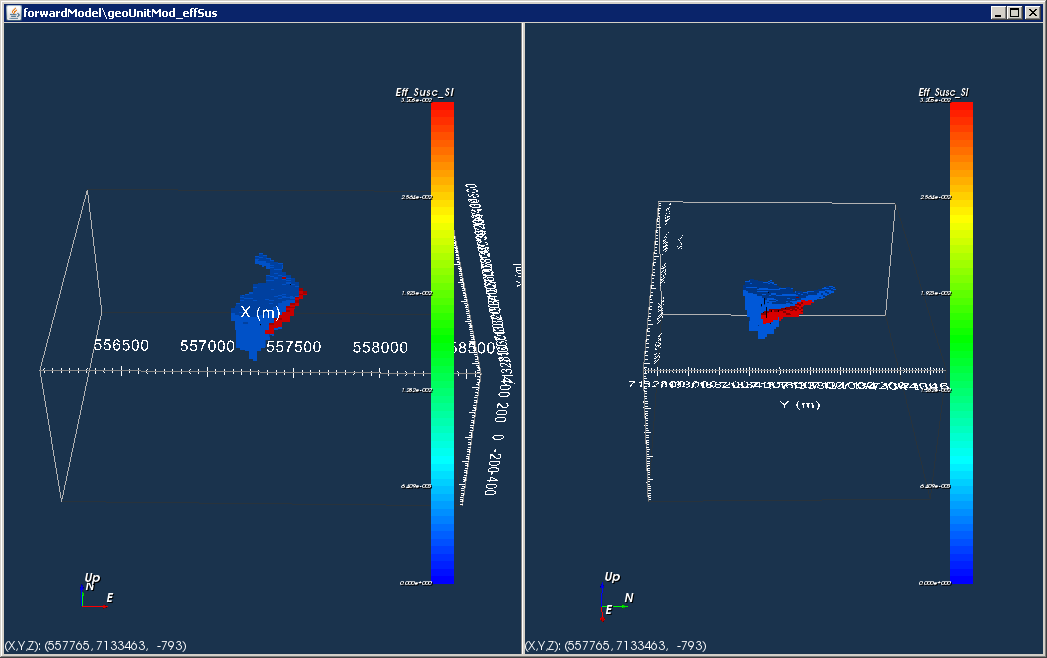
\includegraphics[width=0.8\textwidth]{images/TKC/TKCsuscModel.PNG}
   \caption{effective susceptibility result from voxel-parametric inversion}
   \label{fig:TKCsuscModel}
\end{figure}

Though we do not have oriented \ac{NRM} measurements for TKC samples, the un-oriented \ac{NRM} measurements that we do have added to the measured susceptibilities give us a rough maximum for effective susceptibilities of the  geological in TKC. Given that inversion results imply that the magnetization direction in TKC is close to the earth's field in the location (either show this or cite Sarah's paper), the true  values for effective susceptibilities should be near the maximum value.

Measured maximum effective susceptibility values for HK and PK samples from TKC the results roughly fit petrophysical measurements. The average of measured maximum effective susceptibility for PK is 7.37e-3(SI), and for HK is 0.045(SI) both greater than the recovered values but not so much greater as to imply a very different \ac{NRM} direction from the direction of earth's field.

In terms of the recovered directions of magnetization of the units, the PK unit has an inclination of 83\degree and a declination of 70\degree (an angular difference of 6\degree) and the HK unit has an inclination of 53\degree and a declination of 19\degree (a much larger angular difference of 20\degree).


The fit of this synthetic model to the measured field data is shown in  \autoref{fig:paramModMisfitNorm}, the effective $\Phi_d$ of the predicted data is 
1.01E6 which is significantly higher that the expected value of 7657. This is because the inversion is over-determined rather than under-determined as is the case in most inversions. Since there are so many fewer degrees of freedom than data, the model will only fit the data so well. In addition the voxel-parametric inversion assumes that the geological model provided is completely true while in reality it is only an approximation based on drilling; it also assumes that each unit has a simple, constant property across its extent which is almost certainly untrue.

\begin{figure} [h]
   \centering
   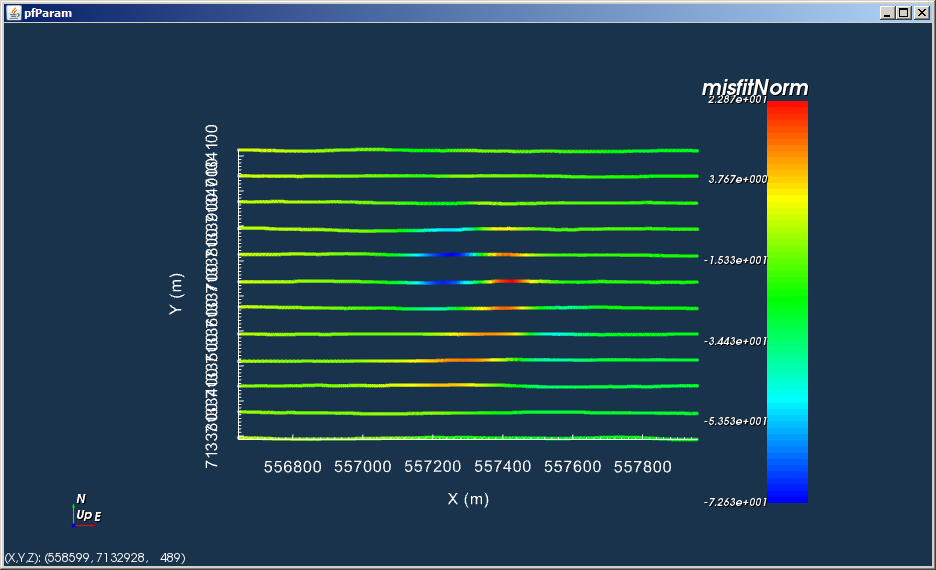
\includegraphics[width=0.8\textwidth]{images/TKC/paramModMisfitNorm.PNG}
   \caption{Normalized misfit of parametric voxel inversion}
   \label{fig:paramModMisfitNorm}
\end{figure}

Given these caveats, the model shown in \autoref{fig:TKCsuscModel} will suit nicely as a sufficiently complex synthetic model for the purposes of showing the capabilities of GIFtools and Model Builder in the performing of inversion on a complicated model with extensive \emph{a priori} information.

To make the inversions easier to preform, the background value (which had an effective susceptibility of 1.09e-3(SI) was set to zero. This avoids having a non-zero reference model in the inversion of the data. the synthetic model with a zero background was forward modeled using the \ac{GIF} \ac{MVI} forward model code. \autoref{fig:Bnoisy} shows the synthetic data contaminated with Gaussian noise with a standard deviation of 1 nanoTesla.

\begin{figure} [h]
   \centering
   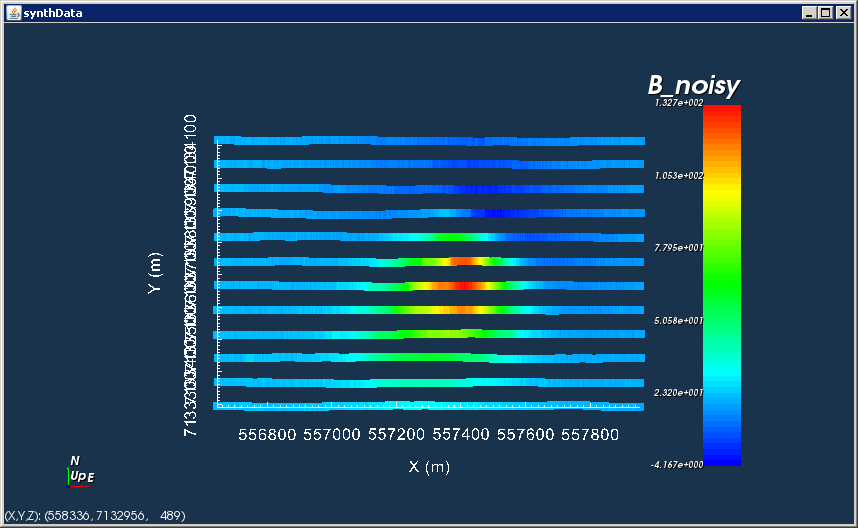
\includegraphics[width=0.8\textwidth]{images/TKC/Bnoisy.PNG}
   \caption{Forward modeled synthetic data contaminated with Gaussian noise}
   \label{fig:Bnoisy}
\end{figure}

The data shown in \autoref{fig:Bnoisy} is the data I will use for the rest of this chapter. It is the predicted data that would be measured over the model shown in \autoref{fig:TKCsuscModel} with a zero background. From this data I will try to recover an anomaly with a similar shape to the model that created the data using various other forms of data (boreholes, cross section maps etc.)


\FloatBarrier
\section{Blind Inversion of the Synthetic Model}
\label{sec:Blind Inversion of the Synthetic Model:TKC}

The inversion whose result is shown in \autoref{fig:blindIndDir} assumes the the magnetization of the anomaly is in the direction of the earth's field. This is not true as discussed in \autoref{sec:Synthetic Model:TKC}. The inversion result highlights the position of the HK unit rather than the PK unit. This is expected given the much higher susceptibility of the HK unit. Since the inversion performed used $L_2$ norms in the \ac{MOF} the model is not compact and over estimates the size of the susceptibility anomaly, especially below the unit in the synthetic model. Additionally, while the position of the HK unit is well estimated at the depth of the true synthetic HK unit, the recovered anomaly dips quite a bit to the south, implying a very different susceptibility distribution than the true synthetic model. By using extra information from \emph{a priori} sources and other inversions I will make the result shown match more closely with the distribution from the synthetic model shown in \autoref{fig:TKCsuscModel}.

\begin{figure}
    \centering
    \begin{subfigure}[b]{0.8\textwidth}
        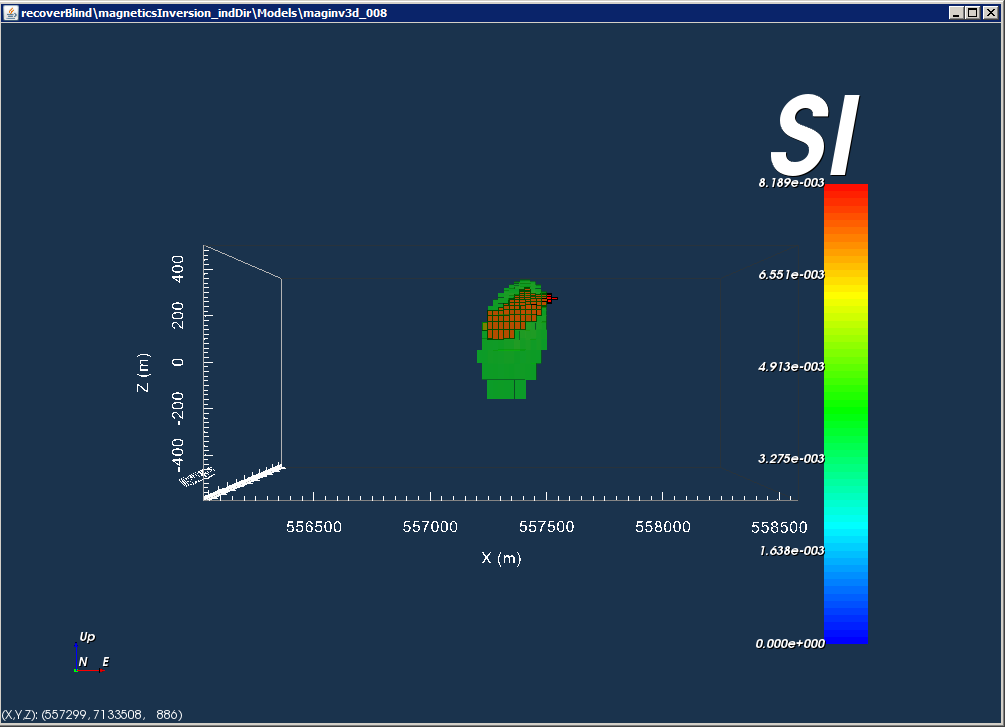
\includegraphics[width=\textwidth]{images/TKC/blindIndDirSouth.PNG}
        \caption{View from south}
        \label{fig:blindIndDirSouth}
    \end{subfigure}
    ~ %add desired spacing between images, e. g. ~, \quad, \qquad, \hfill etc. 
      %(or a blank line to force the subfigure onto a new line)
    \begin{subfigure}[b]{0.8\textwidth}
        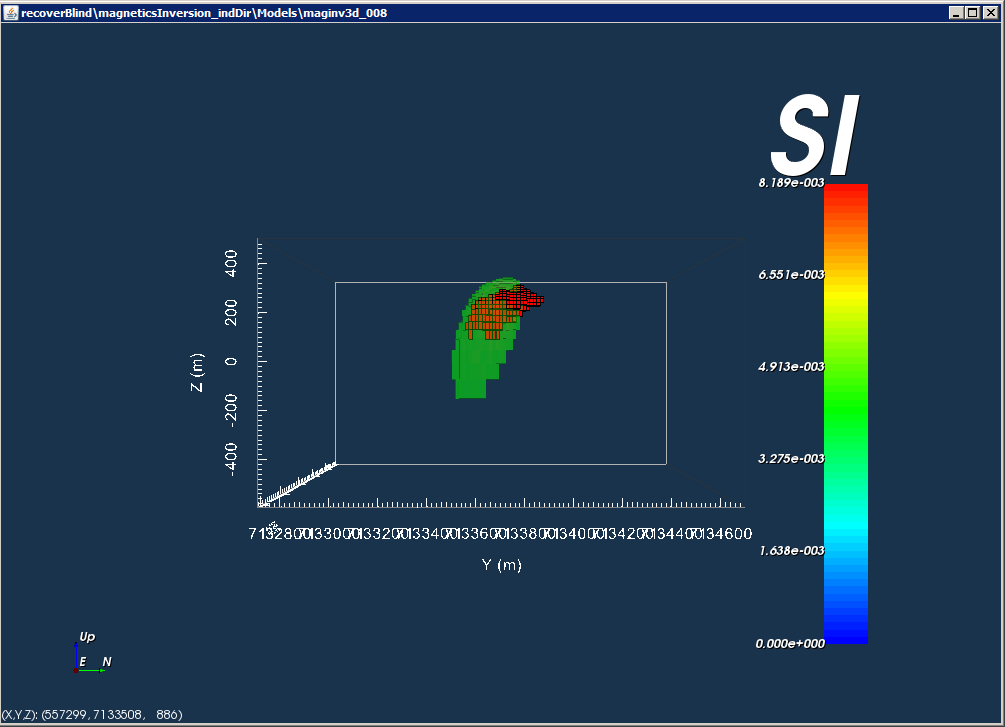
\includegraphics[width=\textwidth]{images/TKC/blindIndDirEast.PNG}
        \caption{View from east}
        \label{fig:blindIndDirEast}
    \end{subfigure}
    ~ %add desired spacing between images, e. g. ~, \quad, \qquad, \hfill etc. 
    %(or a blank line to force the subfigure onto a new line)
   \caption{Blind inversion result assuming a magnetization direction to be the same as the earths field in the location of TKC. (Red cells show the extent of the HK unit in the synthetic model, only cells with a effective susceptibility of greater than 4.0348E-03 (SI) are shown)}
   \label{fig:blindIndDir}
\end{figure}

\FloatBarrier

\section{Determination of Magnetization Direction}
\label{sec:Determination of Magnetization Dirrection}

One of the first pieces of information that can be inserted into the magnetics inversion is the anomalous magnetization direction. \autoref{fig:blind53_19} shows the result when the true magnetization direction of the synthetic HK unit is provided. The result has several advantages over that of the one shown in \autoref{fig:blindIndDir}. While the recovered model still greatly overestimates the size of the susceptibility anomaly below the synthetic HK units, anomaly no longer dips giving a better idea of the lateral position of the susceptibility anomaly. Even at the depth of the synthetic HK unit the lateral position of the anomaly is closer to the synthetic truth.

\begin{figure}
    \centering
    \begin{subfigure}[b]{0.8\textwidth}
        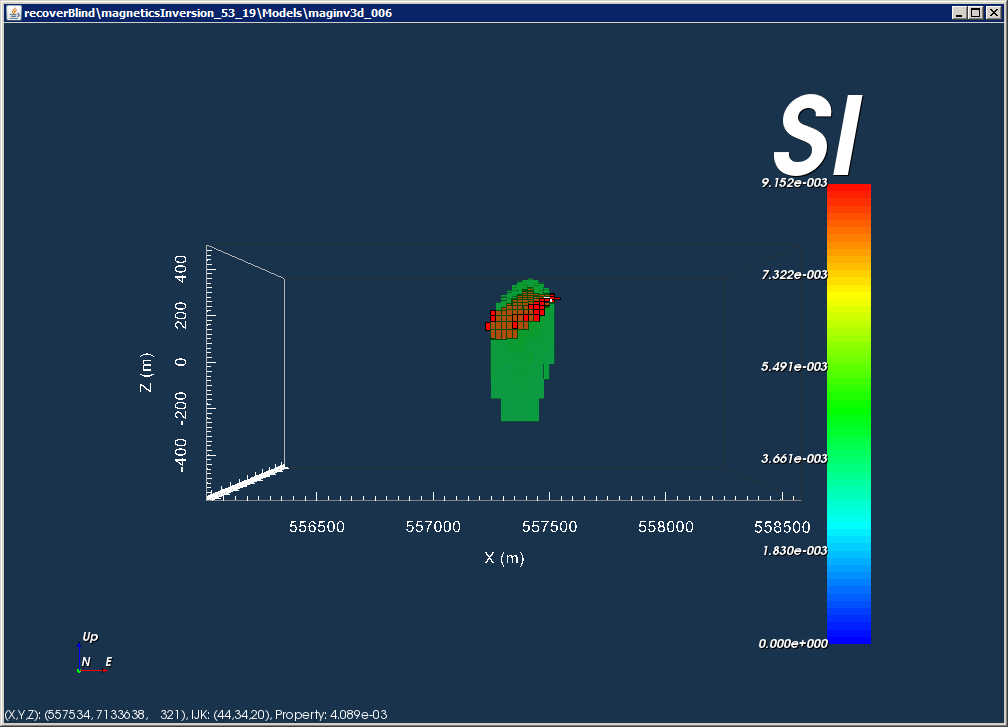
\includegraphics[width=\textwidth]{images/TKC/blind53_19South.PNG}
        \caption{View from south}
        \label{fig:blind53_19South}
    \end{subfigure}
    ~ %add desired spacing between images, e. g. ~, \quad, \qquad, \hfill etc. 
      %(or a blank line to force the subfigure onto a new line)
    \begin{subfigure}[b]{0.8\textwidth}
        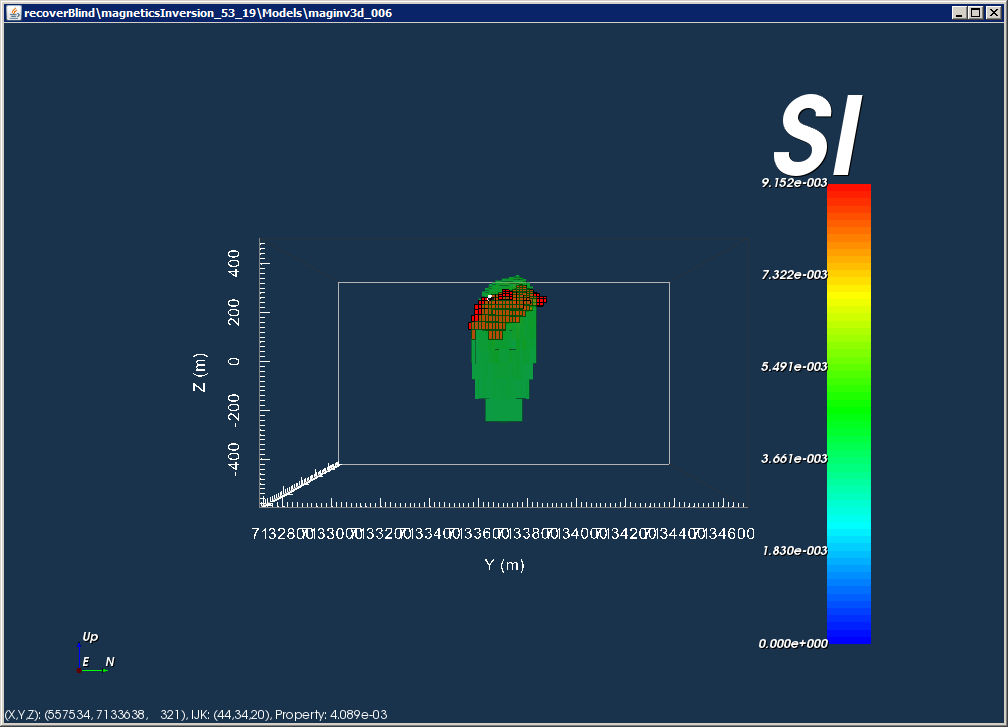
\includegraphics[width=\textwidth]{images/TKC/blind53_19East.PNG}
        \caption{View from east}
        \label{fig:blind53_19East}
    \end{subfigure}
    ~ %add desired spacing between images, e. g. ~, \quad, \qquad, \hfill etc. 
    %(or a blank line to force the subfigure onto a new line)
   \caption{Blind inversion result assuming a magnetization direction to be the magnetization direction of the synthetic HK unit. (Red cells show the extent of the HK unit in the synthetic model, only cells with a effective susceptibility of greater than 4.0348E-03 (SI) are shown)}
   \label{fig:blind53_19}
\end{figure}

Unfortunately we usually don't have the true magnetization direction of an anomaly. For example we do not have the anomaly direction the actual TKC example. To recover the magnetization direction of the anomaly we can use a recovered model using an \ac{MVI} inversion. Using the \ac{GIF} \ac{MVI} code we get the result shown in \autoref{fig:blindMVI} and \autoref{fig:blindMVIFld}. \autoref{fig:blindMVI} shows the magnitude of the magnetization of each model cell normalized by the Earth's field (effective susceptibility). 



\begin{itemize}
  \item we can perform an \ac{MVI} inversion
\end{itemize}

\begin{figure}
    \centering
    \begin{subfigure}[b]{0.8\textwidth}
        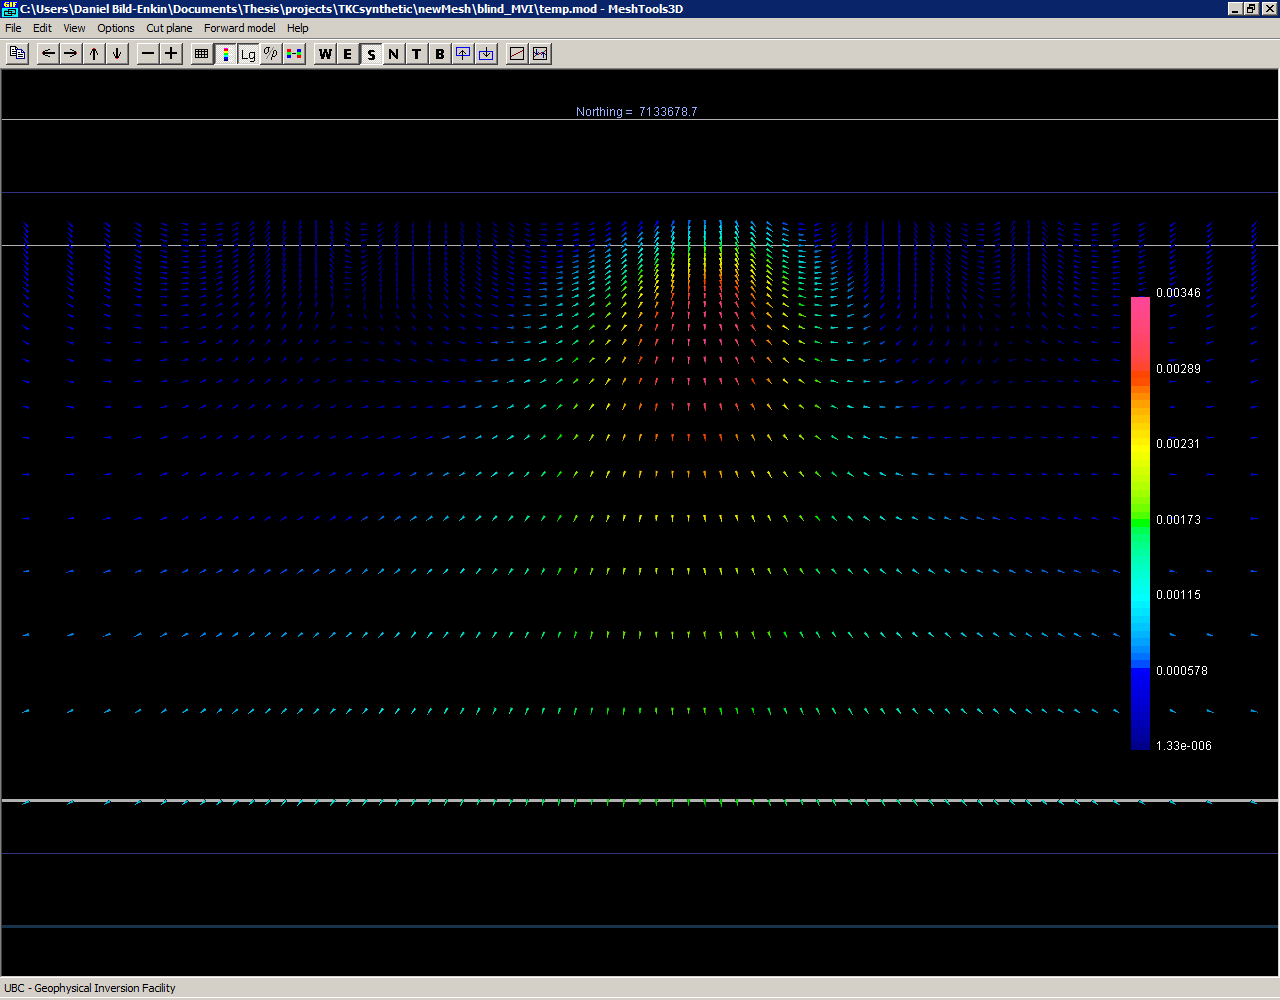
\includegraphics[width=\textwidth]{images/TKC/blindMVIsouth.PNG}
        \caption{View from south}
        \label{fig:blindMVIsouth}
    \end{subfigure}
    ~ %add desired spacing between images, e. g. ~, \quad, \qquad, \hfill etc. 
      %(or a blank line to force the subfigure onto a new line)
    \begin{subfigure}[b]{0.8\textwidth}
        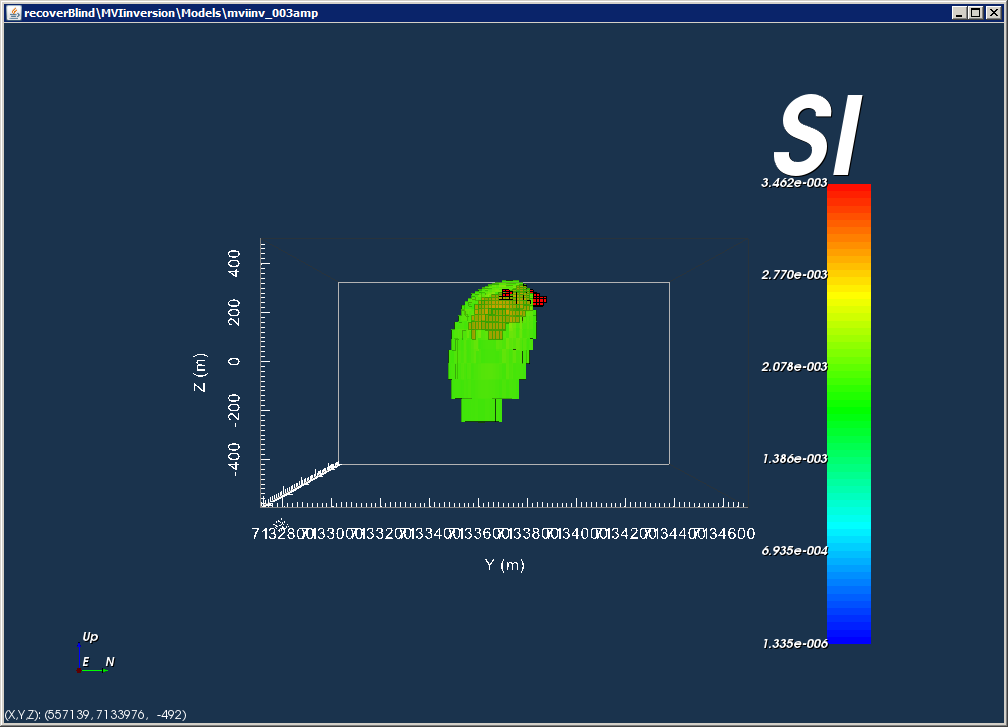
\includegraphics[width=\textwidth]{images/TKC/blindMVIeast.PNG}
        \caption{View from east}
        \label{fig:blindMVIeast}
    \end{subfigure}
    ~ %add desired spacing between images, e. g. ~, \quad, \qquad, \hfill etc. 
    %(or a blank line to force the subfigure onto a new line)
   \caption{Blind inversion amplitude result from the \ac{MVI} code. (Red cells show the extent of the HK unit in the synthetic model, only cells with a effective susceptibility of greater than 2.1039E-03 (SI) are shown)}
   \label{fig:blindMVI}
\end{figure}

\begin{figure}
    \centering
    \begin{subfigure}[b]{0.8\textwidth}
        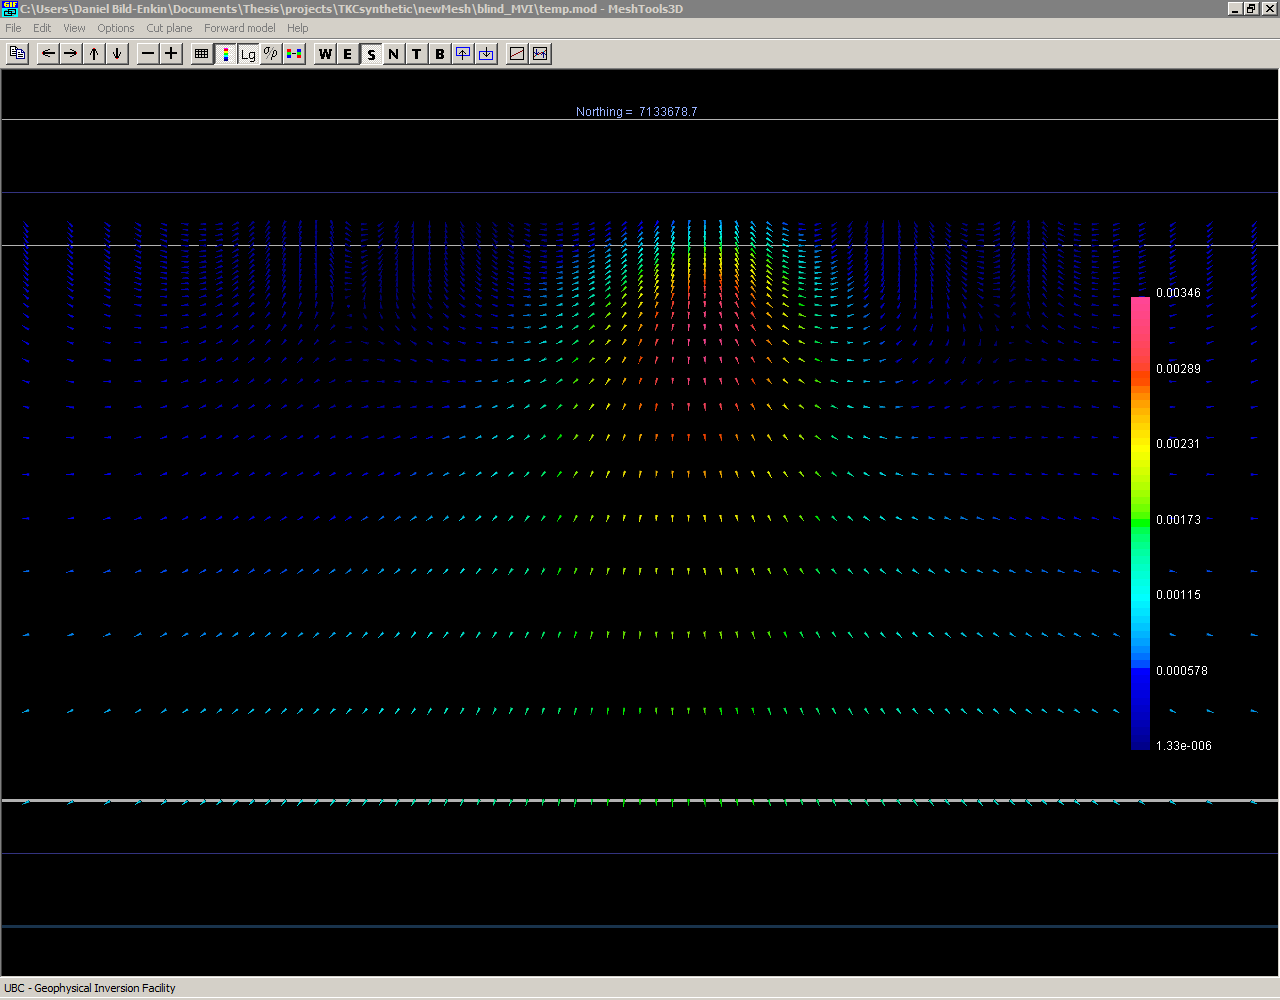
\includegraphics[width=\textwidth]{images/TKC/blindMVIsouthFld.PNG}
        \caption{View from south}
        \label{fig:blindMVIsouthFld}
    \end{subfigure}
    ~ %add desired spacing between images, e. g. ~, \quad, \qquad, \hfill etc. 
      %(or a blank line to force the subfigure onto a new line)
    \begin{subfigure}[b]{0.8\textwidth}
        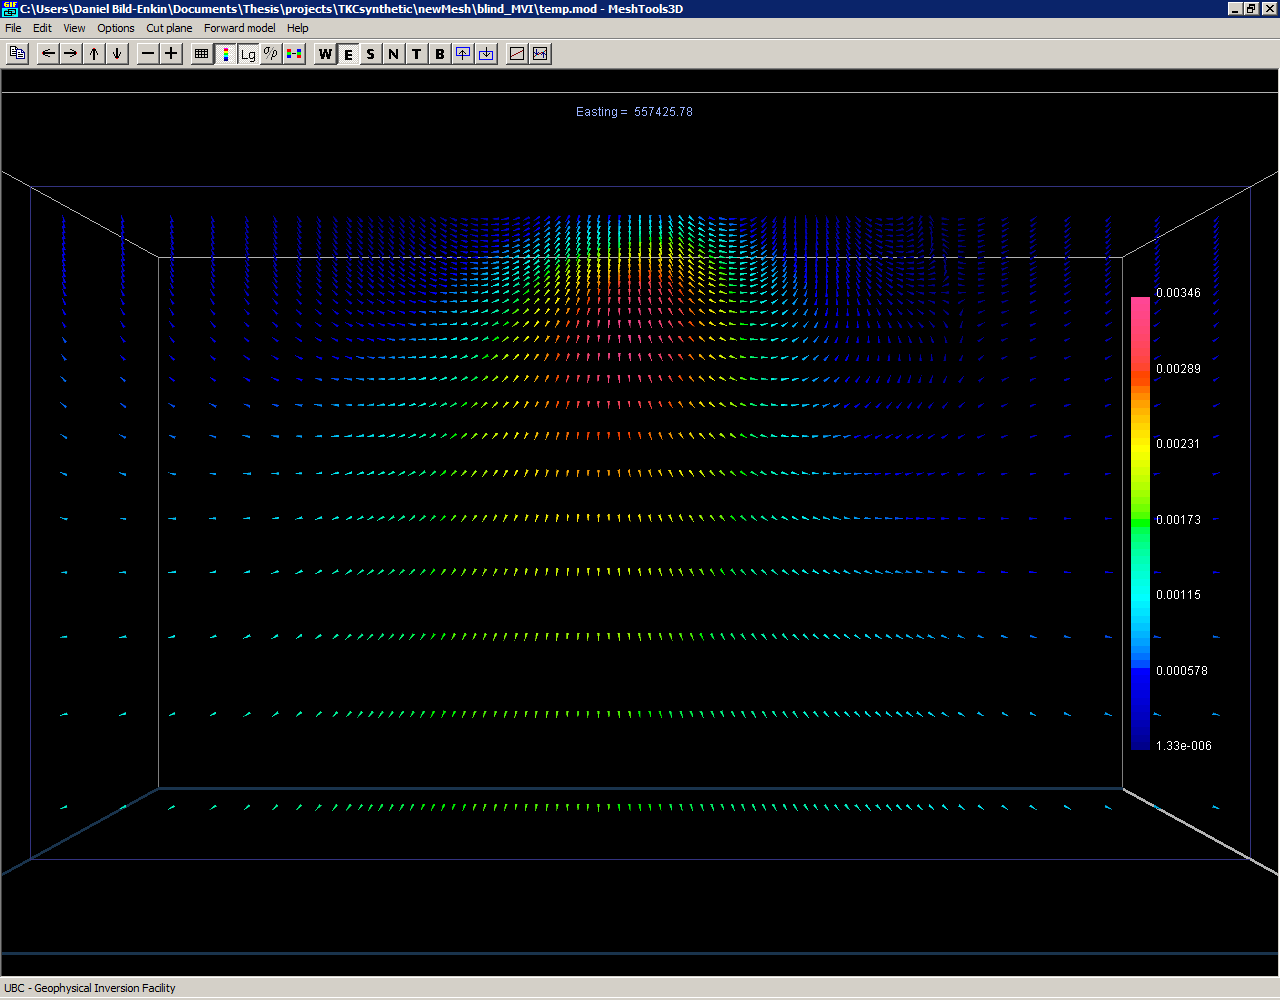
\includegraphics[width=\textwidth]{images/TKC/blindMVIeastFld.PNG}
        \caption{View from east}
        \label{fig:blindMVIeastFld}
    \end{subfigure}
    ~ %add desired spacing between images, e. g. ~, \quad, \qquad, \hfill etc. 
    %(or a blank line to force the subfigure onto a new line)
   \caption{Blind inversion vector result from the \ac{MVI} code. (Red cells show the extent of the HK unit in the synthetic model, only cells with a effective susceptibility of greater than 2.1039E-03 (SI) are shown)}
   \label{fig:blindMVIFld}
\end{figure}




%
%Correlation of Vertical and Total Gradients of Half RTP field \cite{dannemiller2006MagDirection}
%
%taking core direction from MVI result 
%
%apply recovered direction to the anomaly direction in MAG3D
%could also use parametric inversion and MVI sensitivities to provide more constraint.
%
%could apply anomalous dirrection locally to anomaly 
%
%In any case the result will be very similar to the earth's field in the location

\section{Creation of Constraints and Types of Data}
\label{sec:Creation of Constraints:TKC}

%Extensive Boreholes with rock units
%Multiple cross sections (crreated from said bore holes)
%Multiple data types to cluster



\subsection{$\alpha$ coefficients}
\label{sec:alpha coefficients:TKC}

%not much with alphas to be done here given that we don't expect discontinuity in any one particular dirrection.

\subsection{Reference Models}
%\label{sec:Reference Models:TKC}
%
%Most work to be done here. 
%
%We can create a reference model from the phys prop results from the borehole data. Perhaps we should only use some of the boreholes so that we have a more realistic amount of information than in a fully drilled example. We have two ways of applying phys prop measures to inversion and might use both. Also using $K_n$s to improve degree of fit between phys prop measures and effective susc recovered properties
%(show reference model)
%(show result)
%
%with sufficient boreholes we could make a incorrect surface that approximates the ``true'' model used. Use this with parametric inversion for reference model
%(show reference model)
%(show result)
%
%using clustering between density and mag (and conductivity and chargeablity) to create clusters, populate each cluster with a value either the mean value of the cluster or a parametric inversion and use as reference
%(show reference model)
%(show result)
%
%use cross section from \cite{harder2006geologyTKC}
%perhaps extend away from line and down weight
%(show reference model)
%(show result)
%
%(show Combined result)

\subsection{Weighting matrices}
\label{sec:Weighting matrices:TKC}
%
%smallness: using some measure of confidence in the measures decrease in cells with reference model specified to force the result to approximate the reference model. In case the cross section is extended down I will lower the $W_s$ as model cells are further away from the cross section
%(show smallness weight model)
%(show result, compare to result without)
%
%smoothness: to spread the model values away from where they are specified I can increase the smoothness weights in the vicinity of cells with specified reference models. 
%(show face weight model)
%
%with sufficient boreholes we could make a incorrect surface that approximates the ``true'' model used. Use this with parametric inversion for reference mode,l put lower weights along this surface.
%(show face weight model)
%
%using clustering between density and mag (and conductivity and chargeablity) to create clusters, populate each cluster with a value either the mean value of the cluster or a parametric inversion and use as reference
%(show result)
%
%(show result, compare to result without)
%
%(show Combined result)
\subsection{Bounds}
\label{sec:Bounds:TKC}
%
%Also useful for forcing model values to be near the specified reference model while allowing for uncertainty in our phys prop value. Since we have more statistical info on the 
%(show result)
%
%Need to determine if showing the field example is worthwhile at this point and how to bring it into the narrative

\endinput

Any text after an \endinput is ignored.
You could put scraps here or things in progress.
